\pagebreak

\chapter{Using EDIF Cores}

    By 'core' is meant an EDIF netlist file which implements a logic
    function but is not itself a complete logic design.
    
    Note: in the case of the Zynq platform the EDIF file must be a core,
    the bi-directional ports being connected to resources external to the
    FPGA. The CPU interface is incorporated as a large cell called "PS7". 
    
    A Xilinx core EDIF netlist file contains an interface description
    which lists the input and output (and 3-state) connections to the core
    logic. As an example the following core was generated using
    Xilinx coregen -

    \begin{figure}[htbp]
    \centering
    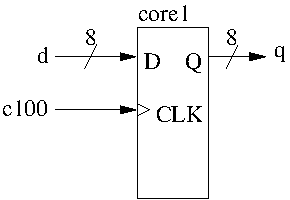
\includegraphics{core1}
    \end{figure}

    This is a simple 8-bit register. The core is called "core2" and
    has the following inputs and outputs -

    \begin{tabular}{l l l}
    port & width & direction \\
    \hline
    D   & 8 & input \\
    CLK & 1 & input \\
    Q   & 8 & output \\
    \end{tabular}

    Note that the use of upper case identifiers for ports seems to be a
    convention with Xilinx but is not required by 3PL.
    
    NGC files are generated from {\bf coregen} via {\bf xst} and are
    linked in by {\bf ngdbuild}.
    
    Note that the core may have an associated constraints file and this can
    be added to a constraints file generated by 3PL by means of library
    procedures {\bf append\_ncf\_file()} \autorefph{sec:lpappncf}.

    \section{linking in EDIF or NGC cores}

        The following 3PL hymod program illustrates how this core can be
        used -
        \begin{lstlisting}[gobble=8, language=threepl]
           module "csiro/hymod/io1.3pl"

           useclock(c100);

           var(ipins, "[]str", {......});
           var(opins, "[]str", {......});
           static(s, "uint:8"); 
           output(,, s, {loc=opins});
           input(d, "uint:8", {loc=ipins});
           value(q, "uint:8");

           import(Q=q <- "core1", CLK=c100, D=d);
           attributes(q, domain=c100);

           s <- q;
        \end{lstlisting}

        Input ports can be driven by expressions or variables of mode
        input, value, static, priority or clock.

        Variables connected to the output ports of the core can only
        be clock, value or selectvalue (for 3-state) mode. Output
        variables to {\bf import()} will not have a clock domain. It may be
        set explicitly by {\bf domain()} as in the example above, otherwise
        variables with no clock domain will not be checked against
        the current clock when evaluated. Note that this does not invalidate
        timing constraints which are set up according to which clocks state
        devices are actually clocked by in the final netlist.
        \index{constraint!timing}
        \index{timing constraint}

        Variables can be arrays or structs.

        The number of bits in each argument must exactly match the
        associated core port width.

        Where a clock is sourced in the core and is connected to the
        main program via {\bf import()} the clock variable must
        be created in the main program, e.g.
        \begin{lstlisting}[gobble=8, language=threepl]
           clock(c, frequency=10e6, tnm="C");
           useclock(c);

           value({d, q}, "uint:8");
           static(s, "uint:8");

           import(Q=q, CLK=c <- "core2", D=d);

           s <- q;
        \end{lstlisting}
        All input ports must be connected but connections to unwanted output
        ports may be omitted.

        To place and route the first example above the procedure is no
        different to usual, e.g.
        \begin{verbatim}
        ngdbuild main
        \end{verbatim}
        Ngdbuild will expect to find a file "core1.edn" which it will link
        in to main.edn.
            
    \section{creating EDIF cores}
    
        To create a core EDIF netlist file the inbuilt procedure {\em export()}
        is called. This generates the interface which enables the core to be
        linked to other EDIF netlist files. As an example -
        \begin{lstlisting}[gobble=8, language=threepl]
           source "xilinx/common.3pl"  // to get declaration of part()
           part("........"); // so core references correct Xilinx element library
           
           clock(c);

           useclock(c);

           static(a, "log");
           static(b, "uint:8");
           value(v1, "log");
           value(v2, "uint:8");

           a <- v1;
           b <- v2;

           export(PA=a, PB=b <- CLK=c, PV1=v1, PV2=v2);
        \end{lstlisting}
        \begin{figure}[htbp]
        \centering
        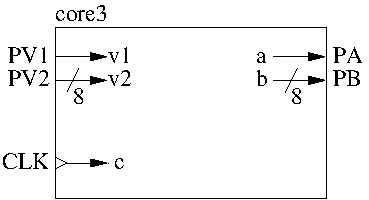
\includegraphics{core3}
        \end{figure}
        In this case {\em PA} and {\em PB} are output ports from this
        core and these are driven by static variables {\em a} and {\em b}.
        The core takes inputs from ports {\em CLK}, {\em PV1} and {\em PV2}.
        The clock variable {\em c} is brought in to the core from outside.
        
        Since the clock {\em c} has an external source we do not have to supply
        a DLL or DCM but we still have to create the clock variable {\em c}
        that is to be connected to the external clock source. The call {\bf
        useclock()} need not precede the {\em export()} call.
        
        The core name must have been supplied using the -e option to the 3PL
        call. This name will also be used for the netlist and constrint outut
        files.
